\documentclass{article} % This command is used to set the type of document you are working on such as an article, book, or presenation

\usepackage[left=0.75in,right=0.75in,top=1cm,bottom=0.5in,%
%includeheadfoot,
headheight=-5pt,headsep=0.4in]{geometry}
\usepackage{graphicx}
\usepackage{dcolumn}
\usepackage{nicefrac}
\usepackage{nomencl}
\usepackage{enumitem}
\usepackage{hyperref}
\usepackage{unicode-math}
\setmathfont{Asana Math}
\usepackage{yfonts}
\usepackage{physics}
\usepackage{titlesec}
\usepackage{xcolor}
\hypersetup{
    colorlinks,
    linkcolor={red!50!black},
    citecolor={blue!50!black},
    urlcolor={blue!80!black}
}
\usepackage{tocdata}
\usepackage{titletoc}
\usepackage{thmbox}

\makenomenclature

\usepackage{geometry}
\usepackage{datetime} 
\usepackage{mathtools}
\usepackage{caption}
\usepackage{exsheets,tasks}
\usepackage{mhchem}

\definecolor{srmorange}{HTML}{EA6A20}
\definecolor{blue}{HTML}{4169E1}
\definecolor{red}{HTML}{DC143C}
\definecolor{green}{HTML}{2E8B57}
\definecolor{mandarin}{HTML}{FF9933}

\newcommand{\red}[1]{\textcolor{red}{#1}} 
\newcommand{\green}[1]{\textcolor{green}{#1}} 
\newcommand{\blue}[1]{\textcolor{blue}{#1}}
\newcommand{\violet}[1]{\textcolor{violet}{#1}}
\newcommand{\gray}[1]{\textcolor{gray}{#1}}
\hypersetup{colorlinks,breaklinks,linkcolor=srmorange,urlcolor=srmorange,anchorcolor=srmorange,citecolor=black}

\newcommand{\maketitletwo}[2][]{\begin{center}
        \textbf{Physics 2}~ 
        (Fall 2025)~
        New Uzbekistan University\\
        contact:~\(\mqty(~\href{mailto:j.kirscher@newuu.uz}{\texttt{j.kirscher@newuu.uz}}\\
        \text{office}~ {\red{\#217}})\)\\            
        \vspace{5pt}
        \hrulefill
        \end{center}}
        
        
\relpenalty=10000
\binoppenalty=70000

\SetupExSheets{
  solution/name=Exercise ,
  headings-format=\itshape\bfseries
}
\settasks{
  counter-format = (\thequestion\alph*) ,
  label-width = 6em
}

\pagestyle{empty}

\begin{document}
\maketitletwo[2]


\begin{question}

Two identical spherical balls with given radii $r$ and masses $m$ are each attached via massless and
infinitely thin strings--such that they cannot not carry any charge--with length $l$ to a common point.

\begin{tasks}(1)
        \task Draw a two-dimensional diagram assuming that gravity acts on the balls and that they are not
        moving.
        \task Find the angle between the strings and the vertical, and draw the force vectors acting on the balls.
\end{tasks}
%
A total charge $Q$ is put onto the balls.

\begin{tasks}(1)
        \task Redraw the diagram to include the Coulomb repulsion between the balls.
        \task Without doing a calculation, argue what fraction of the total charge $Q$ ends up on each ball.\\
        \gray{\small (You might find it helpful to ponder first whether or not the charge distribution is static when the balls
        are not moving or if moving charges can be consistent with a mechanically static situation.)}
        \task Find the new angle between the strings and the vertical for the case when the balls are not moving.
        \task[(bonus)] If \emph{both} balls are displaced by a small arc angle $\phi$ away from the above-considered
        stationary state and then released, what type of motion will the balls perform? 
\end{tasks}
%
Now attach a third ball with identical mass, radius, and charge ($\nicefrac{Q}{2}$) to the same point via a string with length $l$, and
assume that a new stationary equilibrium is reached.

\begin{tasks}(1)
        \task Without doing a calculation, what geometric shape will the three balls form?
        \task Also without a calculation, will the new equilibrium distance between the balls be smaller
        or larger than in the stationary two-ball case?
        \task[(bonus)] For how many balls with charge $\nicefrac{Q}{2}$ attached to the same point with rigid strings of length $l$
        will the distance between neighboring balls be maximal before the addition of another ball leads to a
        smaller distance between neighboring balls?
\end{tasks}

\end{question}

\begin{question}
        Consider an ``atomic chess board'' on which each figure type is represented by a different atom:
        \[
        \mqty(~
        \text{King} & \text{Queen} & \text{Bishop} & \text{Knight} & \text{Rook} & \text{Pawn}~ \\
        \ce{^{79}Au}& \ce{^{78}Pt} & \ce{^{14}Si} & \ce{^{29}Cu} & \ce{^{26}Fe} & \ce{^{1}H}
        )
        \qq{.}
        \]
        The number of ``valence'' electrons as indicated by the small orbiting dots in the figure, e.g.,
        ten for $\ce{^{78}Pt}$, indicates by how much the atom/figure is ionized when moved from its starting
        position. For example, during the initial move \texttt{E2E4}, the pawn/\ce{^{1}H}-atom looses its
        only electron and ends as a proton, i.e., a hydrogen ion, on the
        field \texttt{E4}.

        Let the atoms always be fixed at the center of their respective fields, and assume that
        the width of the fields is $l = 1$cm.
        \begin{tasks}(1)
                \task Without calculation, what is the electrostatic potential energy of the initial configuration?
                \task \emph{Discuss} (do not calculate) the change in the electrostatic potential ($U_\texttt{E2E4}$)
                 energy after an initial \texttt{E2E4} move.
                \task Again without calculation is how does the change in potential for an alternative opening
                move \texttt{D1C3} compare to the one for \texttt{E2E4}:
                \[
                U_\texttt{B1C3} - U_\texttt{E2E4} \stackrel{?}{\gtreqqless}0 \qq{.}
                \]
        \end{tasks}
        

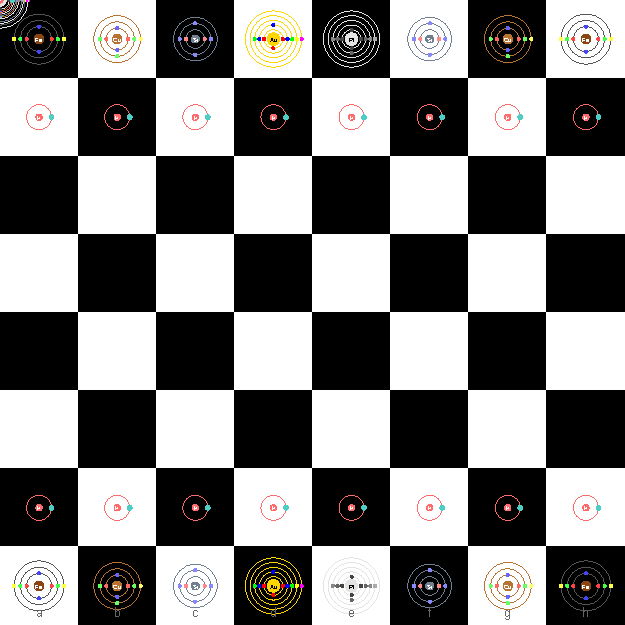
\includegraphics[width=1.\textwidth]{atomic_chess_board.pdf}

\end{question}

\printnomenclature

%\renewcommand\bibname{Reference}
\renewcommand\refname{Recommended Reading}

\nocite{*}
\bibliographystyle{plain}
\bibliography{problem.bib}

\end{document}